\chapter{Implementation and Compilation Model}

\section{Implementation Overview}

This section provides a foundation for all subsequent sections by describing the host language, the overall architecture of the GG-Code compiler, the five-stage pipeline through which source code is transformed into G-code, and the key design decisions made during development.

\subsection*{Host Language and Toolchain}

GG-Code is implemented entirely in \textbf{Python 3}, which serves as the sole implementation language across every stage of the compilation pipeline. The choice of Python was motivated by three considerations. First, ANTLR4 provides an officially supported Python3 runtime, allowing the generated lexer and parser to be used directly within the project without any cross-language bridging. Second, Python's dataclass mechanism provides a concise and readable way to define the typed AST nodes that form the backbone of the compiler's intermediate representation. Third, Python's standard library and the availability of the \texttt{antlr4-python3-runtime} and \texttt{fastapi} packages allowed the entire toolchain, including the web backend, to be built within a single language ecosystem.

The toolchain consists of two layers. The first is \textbf{ANTLR4}, which reads the grammar file \texttt{src/grammar/GGCode.g4} and automatically generates the lexer, parser, visitor base class, and listener base class into the \texttt{src/antlr\_gen/} directory. These generated files are never edited manually. The second layer is the hand-written Python implementation, which provides the AST node definitions, the AST builder, the semantic analyzer, and the code generator. The entry point for the compiler is \texttt{src/main.py}, which exposes the function \texttt{run\_pipeline}.

\subsection*{Pipeline Architecture}

The processing of a GG-Code program follows a linear five-stage pipeline, illustrated in Figure~\ref{fig:impl_pipeline}. Each stage transforms the program into a representation suitable for the next stage, beginning with raw source text and ending with a valid G-code string.

Execution begins in \texttt{run\_pipeline}, which receives the source code as a string. The source is wrapped in ANTLR4's \texttt{InputStream} and passed to the lexer. The resulting token stream is then consumed by the parser, which produces a parse tree. An \texttt{ASTBuilder} visitor traverses the parse tree and constructs a typed, Python-dataclass-based Abstract Syntax Tree. The \texttt{SemanticAnalyzer} then walks the AST to validate scoping, variable declarations, and named-location references. Finally, the \texttt{GCodeGenerator} traverses the validated AST and emits G-code instructions, returning the complete G-code program as a string.

\begin{figure}[H]
\centering
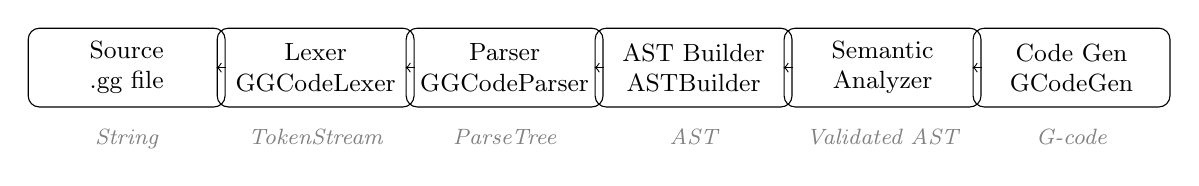
\begin{tikzpicture}[
  node distance=2.4cm,
  box/.style={draw, rounded corners, minimum width=2.5cm, minimum height=1.0cm, align=center, font=\small},
  note/.style={font=\footnotesize\itshape, text=gray}
]
\node[box] (src)  {Source\\.gg file};
\node[box] (lex)  [right of=src]  {Lexer\\GGCodeLexer};
\node[box] (par)  [right of=lex]  {Parser\\GGCodeParser};
\node[box] (ast)  [right of=par]  {AST Builder\\ASTBuilder};
\node[box] (sem)  [right of=ast]  {Semantic\\Analyzer};
\node[box] (gen)  [right of=sem]  {Code Gen\\GCodeGen};

\draw[->] (src) -- (lex);
\draw[->] (lex) -- (par);
\draw[->] (par) -- (ast);
\draw[->] (ast) -- (sem);
\draw[->] (sem) -- (gen);

\node[note] at (src.south)  [below=0.15cm] {String};
\node[note] at (lex.south)  [below=0.15cm] {TokenStream};
\node[note] at (par.south)  [below=0.15cm] {ParseTree};
\node[note] at (ast.south)  [below=0.15cm] {AST};
\node[note] at (sem.south)  [below=0.15cm] {Validated AST};
\node[note] at (gen.south)  [below=0.15cm] {G-code};
\end{tikzpicture}
\caption{Five-stage GG-Code compilation pipeline}
\label{fig:impl_pipeline}
\end{figure}

Unlike a traditional interpreter, the GG-Code compiler does not execute the program. Instead, it statically unrolls all control flow that can be evaluated at compile time (such as \texttt{Repeat N times}) and emits the corresponding G-code instructions. The output is a standalone \texttt{.gcode} file that can be sent directly to any compatible 3D printer or CNC machine without any runtime support.

\subsection*{Design Philosophy: Compilation over Interpretation}

The decision to compile GG-Code to G-code rather than interpret it directly reflects the execution model of the target domain. G-code files are stored on SD cards or transferred to machine controllers that have no runtime environment. The compiler must therefore resolve all control flow statically and produce a flat sequence of machine instructions. For constructs that cannot be resolved statically, such as \texttt{While} loops whose termination depends on a dynamic condition, the compiler emits the loop body once and annotates it with a warning comment, acknowledging the fundamental limitation of targeting a non-Turing-complete output format.

\subsection*{Project File Structure}

The repository is organized as follows:

\begin{center}
\begin{tabular}{|l|p{9cm}|}
\hline
\textbf{File / Directory} & \textbf{Role} \\
\hline
\texttt{src/grammar/GGCode.g4} & ANTLR4 grammar defining all lexer and parser rules for GG-Code \\
\hline
\texttt{src/antlr\_gen/} & Auto-generated directory: \texttt{GGCodeLexer.py}, \texttt{GGCodeParser.py}, \texttt{GGCodeVisitor.py}, \texttt{GGCodeListener.py} \\
\hline
\texttt{src/main.py} & Entry point and \texttt{run\_pipeline} function; also handles CLI argument parsing \\
\hline
\texttt{src/parser/antlr\_converter.py} & \texttt{ASTBuilder} class: ANTLR4 visitor that transforms the parse tree into typed Python dataclass AST nodes \\
\hline
\texttt{src/ast\_nodes/} & Dataclass definitions for all AST node types: \texttt{base.py}, \texttt{program.py}, \texttt{statements.py}, \texttt{expressions.py} \\
\hline
\texttt{src/semantic/} & \texttt{SemanticAnalyzer}, \texttt{SymbolTable}, and \texttt{SemanticError} \\
\hline
\texttt{src/codegen/gcode\_generator.py} & \texttt{GCodeGenerator}: walks the AST and emits G-code lines \\
\hline
\texttt{src/lexer/token\_types.py} & \texttt{TokenType} enum used by expressions and the code generator for operator dispatch \\
\hline
\texttt{backend/server.py} & FastAPI web server exposing \texttt{/compile} and \texttt{/upload} endpoints \\
\hline
\texttt{frontend/} & React + TypeScript web IDE with Monaco editor and Three.js 3D G-code visualizer \\
\hline
\texttt{tests/test\_pipeline.py} & pytest integration tests that call \texttt{run\_pipeline} end-to-end \\
\hline
\end{tabular}
\end{center}

\subsection*{Relationship Between Stages}

The five stages are tightly coupled through shared data structures. The ANTLR4 parse tree is the interface between the parser and the \texttt{ASTBuilder}. The Python dataclass AST is the interface between the \texttt{ASTBuilder} and both the \texttt{SemanticAnalyzer} and the \texttt{GCodeGenerator}. Any change to the grammar requires regenerating the \texttt{src/antlr\_gen/} directory and potentially updating the corresponding visitor methods in \texttt{ASTBuilder}. Any change to the AST node definitions requires updating both the \texttt{ASTBuilder} (which creates nodes) and the \texttt{GCodeGenerator} (which consumes them).

% ─────────────────────────────────────────────────────────────────────────────
\section{Toolchain: ANTLR4}

The GG-Code compiler relies on ANTLR4 (Another Tool for Language Recognition, version~4) as its parser-generator framework. ANTLR4 is an open-source tool that accepts a grammar in its own notation and automatically produces a lexer, a parser, and supporting traversal interfaces in the target host language. In the case of GG-Code, the target is Python~3.

\subsection*{Role in the Toolchain}

ANTLR4 is responsible for the first two stages of the GG-Code pipeline. Given the grammar file \texttt{GGCode.g4}, ANTLR4 generates four artefacts into the \texttt{src/antlr\_gen/} directory:

\begin{description}
    \item[-][\texttt{GGCodeLexer.py}] -- Lexical analyser generated from the token rules defined in the grammar. It converts a character stream into a token stream.
    \item[-][\texttt{GGCodeParser.py}] -- Syntactic analyser generated from the parser rules. It consumes the token stream and constructs a concrete parse tree.
    \item[-][\texttt{GGCodeVisitor.py}] -- Visitor base class providing a \texttt{visit} method for every parser rule. The \texttt{ASTBuilder} class subclasses this.
    \item[-][\texttt{GGCodeListener.py}] -- Listener base class with \texttt{enter}/\texttt{exit} hooks for every parser rule (unused in the current implementation).
\end{description}

None of these files are edited manually. They are regenerated whenever the grammar changes by invoking the ANTLR4 tool-jar:

\begin{center}
\verb|java -jar antlr-4.9.3-complete.jar -Dlanguage=Python3 -visitor -o src/antlr_gen src/grammar/GGCode.g4|
\end{center}

\subsection*{Parser Strategy: Adaptive LL(*)}

The parser generated by ANTLR4 uses the \textbf{Adaptive LL(*)} parsing algorithm~\cite{parr_adaptive_2011}. The algorithm belongs to the family of top-down parsers: it begins at the root production rule (\texttt{program}) and recursively expands rules from left to right. At each decision point it looks ahead in the token stream by as many tokens as necessary to resolve the ambiguity, adapting its lookahead dynamically. This is well suited to the GG-Code grammar, where the leading keyword of each statement (e.g.\ \texttt{MOVE}, \texttt{REPEAT}, \texttt{IF}) provides strong predictive cues that allow early disambiguation without backtracking.

\subsection*{Why ANTLR4 Was Chosen}

Several factors led to the selection of ANTLR4 over alternatives such as PLY (Python Lex-Yacc) or a hand-written recursive-descent parser.

First, ANTLR4 generates both the lexer and parser from a single unified grammar file, keeping the formal specification of the language in one place. Second, the generated parser produces a typed parse tree in which every node is an instance of a context class named after the grammar rule that produced it. This makes it straightforward to subclass the generated visitor and dispatch on specific node types inside \texttt{ASTBuilder}. Third, ANTLR4's Python3 runtime is mature and introduces negligible overhead for the scale of programs GG-Code is designed to compile.

\subsection*{Separation of Generated and Hand-Written Code}

A deliberate architectural decision was made to isolate all generated code in the \texttt{src/antlr\_gen/} directory and import it only from \texttt{src/main.py} and \texttt{src/parser/antlr\_converter.py}. This ensures that regenerating the grammar does not affect any other module. The \texttt{ASTBuilder} depends on the context classes produced by ANTLR4 to identify node types, but it does not extend the generated listener. Instead, it implements the visitor interface by overriding specific \texttt{visit*} methods, one per grammar rule.

% ─────────────────────────────────────────────────────────────────────────────
\section{Lexical Analysis}

The lexical analysis stage transforms the raw source character stream into a structured sequence of typed tokens. In GG-Code this stage is handled entirely by \texttt{GGCodeLexer}, the lexer generated by ANTLR4 from the lexical rules defined in \texttt{GGCode.g4}.

ANTLR4 generates a deterministic finite automaton (DFA)-based lexical analyser that scans the source sequentially and applies pattern-matching rules. Each recognised token is emitted into a \texttt{CommonTokenStream}, which is then consumed by the parser.

GG-Code defines the following categories of lexical tokens:

\begin{itemize}
    \item[-] \textbf{Keywords:} Motion control (\texttt{MOVE}, \texttt{HOME}, \texttt{STOP}, \texttt{PAUSE}), machine control (\texttt{TEMPERATURE}, \texttt{WAIT}, \texttt{USE}), geometry (\texttt{ADD}, \texttt{SQUARE}, \texttt{CIRCLE}, \texttt{RECTANGLE}, \texttt{LINE}), definitions (\texttt{DEFINE}, \texttt{SET}), and control flow (\texttt{IF}, \texttt{THEN}, \texttt{ELSE}, \texttt{REPEAT}, \texttt{WHILE}).
    \item[-] \textbf{Axis Values:} Tokens of the form \texttt{X10}, \texttt{Y-5.5}, \texttt{Z0.2} that combine an axis letter with a signed numeric value, recognised by the \texttt{AXIS\_VALUE} rule.
    \item[-] \textbf{Temperature Values:} Tokens of the form \texttt{200C} recognised by the \texttt{TEMPERATURE\_VALUE} rule.
    \item[-] \textbf{Measure Values:} Tokens of the form \texttt{20mm} or \texttt{2.5cm} recognised by the \texttt{MEASURE} rule.
    \item[-] \textbf{Numeric Literals:} Integer tokens (\texttt{INTERGER}) and decimal tokens (\texttt{DECIMAL}).
    \item[-] \textbf{Identifiers:} User-defined names for variables and locations, recognised by \texttt{IDENTIFIER}.
    \item[-] \textbf{Operators and Delimiters:} Arithmetic operators, comparison operators, parentheses, and braces.
\end{itemize}

\subsection*{Case-Insensitive Keywords}

A distinctive feature of the GG-Code grammar is that all keywords are defined as case-insensitive character class alternations in ANTLR4. For example:

\begin{center}
\verb|MOVE: [Mm][Oo][Vv][Ee];|
\end{center}

This means that \texttt{Move}, \texttt{MOVE}, and \texttt{move} are all recognised as the same keyword token. This design decision was motivated by the domain: manufacturing engineers and hobbyists are accustomed to writing commands in various capitalisation styles, and requiring strict casing would create unnecessary friction.

\subsection*{Tokenization Example}

The following GG-Code instruction:

\begin{center}
\verb|Move to X10 Y20|
\end{center}

is transformed into the token sequence shown in Figure~\ref{fig:lexer-example}.

\begin{figure}[H]
\centering
\begin{tabular}{|c|c|}
\hline
\textbf{Lexeme} & \textbf{Token Type} \\
\hline
\texttt{Move}  & \texttt{MOVE} \\
\texttt{to}    & \texttt{TO} \\
\texttt{X10}   & \texttt{AXIS\_VALUE} \\
\texttt{Y20}   & \texttt{AXIS\_VALUE} \\
\hline
\end{tabular}
\caption{Example lexical tokenization for a Move statement}
\label{fig:lexer-example}
\end{figure}

\subsection*{Priority and Longest-Match Resolution}

When multiple lexer rules can match the same input, ANTLR4 applies the longest-match strategy first. If multiple rules match the same number of characters, priority is determined by the order of rule definitions in the grammar. In GG-Code this matters for disambiguation between keywords and identifiers: for example, the lexeme \texttt{Set} would match both the \texttt{SET} keyword rule and the general \texttt{IDENTIFIER} rule. Because \texttt{SET} is defined before \texttt{IDENTIFIER} in the grammar, it takes priority.

\subsection*{Whitespace and Comment Handling}

Whitespace (spaces, tabs, and newlines) is sent to the hidden ANTLR4 channel and never reaches the parser:

\begin{center}
\verb|WS: [ \t\r\n]+ -> skip;|
\end{center}

Both C-style line comments (\verb|// ...|) and block comments (\verb|/* ... */|) are similarly discarded:

\begin{center}
\verb|LINE_COMMENT: '//' ~[\r\n]* -> skip;| \\
\verb|BLOCK_COMMENT: '/*' .*? '*/' -> skip;|
\end{center}

This means that comments have no representation in the token stream and are not visible to any downstream stage.

% ─────────────────────────────────────────────────────────────────────────────
\section{Syntactic Analysis}

The syntactic analysis stage verifies that the sequence of tokens produced by the lexer conforms to the grammatical structure of GG-Code. During this phase, the \texttt{GGCodeParser} consumes the \texttt{CommonTokenStream} and constructs a hierarchical parse tree that represents the syntactic structure of the program.

The grammar of GG-Code is context-free and supports recursive constructs, particularly in expression evaluation and nested block statements. The generated parser uses the Adaptive LL(*) strategy described in Section~3.2.

\subsection*{Parser Workflow}

Parsing begins at the entry rule:

\begin{center}
\verb|parser.program()|
\end{center}

The \texttt{program} rule is defined as a \texttt{statementList} followed by \texttt{EOF}. The object returned is an instance of \texttt{GGCodeParser.ProgramContext}, which serves as the root of the parse tree. Figure~\ref{fig:parser-pipeline} illustrates the relationship between lexical and syntactic analysis.

\begin{figure}[H]
\centering
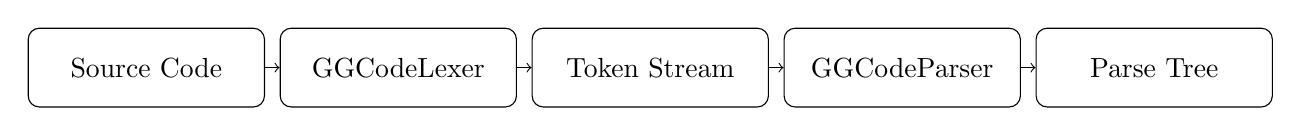
\begin{tikzpicture}[
node distance=3.2cm,
every node/.style={draw, rounded corners, minimum width=3cm, minimum height=1cm, align=center}
]
\node (source) {Source Code};
\node (lexer) [right of=source] {GGCodeLexer};
\node (tokens) [right of=lexer] {Token Stream};
\node (parser) [right of=tokens] {GGCodeParser};
\node (tree) [right of=parser] {Parse Tree};
\draw[->] (source) -- (lexer);
\draw[->] (lexer) -- (tokens);
\draw[->] (tokens) -- (parser);
\draw[->] (parser) -- (tree);
\end{tikzpicture}
\caption{Lexical and syntactic analysis pipeline}
\label{fig:parser-pipeline}
\end{figure}

\subsection*{Grammar Structure}

The grammar organizes all statements into two categories. \textbf{Simple statements} cover the four statement families: motion commands (\texttt{moveStatement}, \texttt{homeStatement}, \texttt{stopStatement}, \texttt{pauseStatement}), machine commands (\texttt{temperatureStatement}, \texttt{waitStatement}, \texttt{useStatement}), geometry commands (\texttt{squareStatement}, \texttt{rectangleStatement}, \texttt{circleStatement}, \texttt{lineStatement}), and definition commands (\texttt{defineStatement}, \texttt{setStatement}). \textbf{Compound statements} cover the control flow constructs: \texttt{conditionalStatement}, \texttt{loopStatement}, and \texttt{blockStatement}.

\subsection*{Expression Grammar and Operator Precedence}

Arithmetic and comparison expressions are represented through a hierarchy of grammar rules that encodes operator precedence explicitly. From lowest to highest precedence:

\begin{center}
\texttt{comparisonExpression} $\supset$ \texttt{additiveExpression} $\supset$ \texttt{multiplicativeExpression} $\supset$ \texttt{unaryExpression} $\supset$ \texttt{primaryExpression}
\end{center}

Each level uses a ``tail'' production to allow left-associative repetition without introducing left recursion. For example:

\begin{center}
\verb|additiveExpression: multiplicativeExpression additiveTail;|\\
\verb|additiveTail: addOperator multiplicativeExpression additiveTail | ;|
\end{center}

This structure allows expressions such as \texttt{3 + 4 * 2} to be parsed with multiplication binding more tightly than addition, and the \texttt{ASTBuilder} reconstructs left-associative binary expression trees from the resulting right-recursive tail nodes.

\subsection*{Syntax Error Detection}

When the token stream violates the grammar, ANTLR4 generates a syntax error and reports its location. The \texttt{run\_pipeline} function checks \texttt{parser.getNumberOfSyntaxErrors()} immediately after parsing and raises a \texttt{SyntaxError} if any errors were detected, terminating compilation before AST construction begins. Common syntax errors include:

\begin{itemize}
    \item[-] Missing \texttt{TO} keyword after \texttt{MOVE}
    \item[-] Malformed axis value (e.g., a bare \texttt{X} without a number)
    \item[-] Unclosed braces in block statements
    \item[-] Incomplete expressions in \texttt{If} or \texttt{While} conditions
\end{itemize}

% ─────────────────────────────────────────────────────────────────────────────
\section{AST Construction}

After syntactic analysis, the \texttt{ASTBuilder} class in \texttt{src/parser/antlr\_converter.py} transforms the ANTLR4 parse tree into a typed Abstract Syntax Tree composed of Python dataclass nodes. This intermediate representation is simpler than the parse tree: it discards syntactic punctuation (braces, keywords used only as delimiters), makes semantic relationships explicit as typed fields, and forms the input to both the semantic analyzer and the code generator.

\subsection*{Role of the Typed AST}

The ANTLR4 parse tree preserves every syntactic detail, including intermediate grammar rule nodes, delimiter tokens, and redundant structure introduced by the tail productions used to avoid left recursion. The typed AST strips this syntactic noise and retains only the semantically meaningful structure. For instance, the tail-recursive chain produced by the expression grammar for \texttt{3 + 4 * 2} is collapsed into a nested \texttt{BinaryExpression(BinaryExpression(Literal(3), PLUS, Literal(4)), STAR, Literal(2))} tree by the \texttt{\_processAdditiveTail} helper in \texttt{ASTBuilder}.

\subsection*{The \texttt{ASTBuilder} Visitor}

\texttt{ASTBuilder} subclasses the generated \texttt{GGCodeVisitor} and overrides a \texttt{visit*} method for each grammar rule that requires transformation. The central dispatch is provided by ANTLR4's \texttt{visit(ctx)} method, which automatically calls the appropriate overridden method based on the runtime type of the context node.

Each \texttt{visit*} method returns a typed AST node or a plain Python dictionary (for intermediate constructs such as move targets). For example, \texttt{visitMoveStatement} returns a \texttt{MoveStatement} node whose \texttt{target} field holds a dict such as \texttt{\{'type': 'axis\_pair', 'values': ['X10', 'Y20']\}}. This lightweight dict approach was chosen for move targets because the variety of valid target forms (single axis, axis pair, axis triplet, named location, predefined point) makes it more practical to dispatch on a string type tag in the code generator than to define a separate AST node class for each variant.

\subsection*{AST Node Hierarchy}

All AST nodes are Python \texttt{@dataclass} subclasses of \texttt{ASTNode} (defined in \texttt{src/ast\_nodes/base.py}), which carries \texttt{line} and \texttt{column} attributes for error reporting. The node hierarchy is organized into three modules:

\begin{itemize}
    \item[-] \textbf{\texttt{program.py}}: The root \texttt{Program} node, which holds a list of top-level statements.
    \item[-] \textbf{\texttt{statements.py}}: All statement node types, including \texttt{MoveStatement}, \texttt{IfStatement}, \texttt{RepeatStatement}, \texttt{WhileStatement}, \texttt{TemperatureStatement}, \texttt{WaitStatement}, \texttt{SetStatement}, \texttt{DefineStatement}, \texttt{AddShapeStatement}, \texttt{HomeStatement}, \texttt{StopStatement}, \texttt{PauseStatement}, and \texttt{Block}.
    \item[-] \textbf{\texttt{expressions.py}}: Expression node types: \texttt{Literal}, \texttt{Identifier}, \texttt{BinaryExpression}, \texttt{UnaryExpression}.
\end{itemize}

Figure~\ref{fig:ast-example} shows the parse tree generated for a \texttt{Repeat} loop, which serves as the structural input for AST construction.

\begin{figure}[H]
\centering
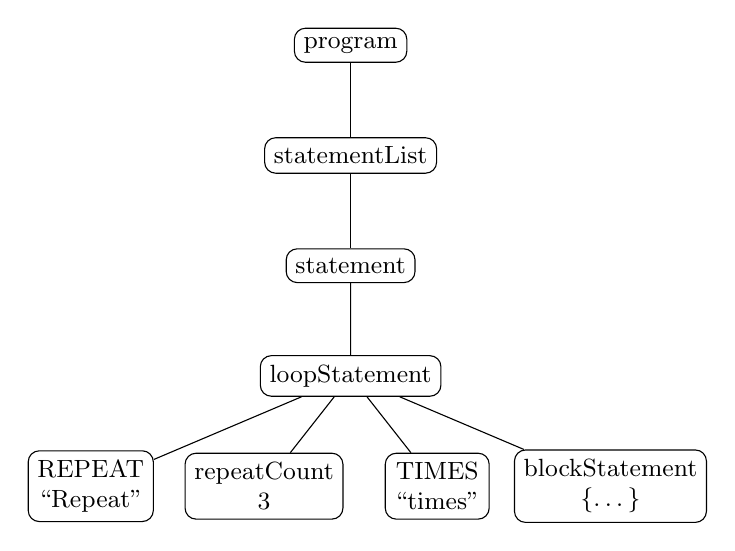
\begin{tikzpicture}[
level distance=1.4cm,
level 1/.style={sibling distance=6.5cm},
level 2/.style={sibling distance=3.2cm},
level 3/.style={sibling distance=2.2cm},
every node/.style={draw, rounded corners, align=center, font=\small}
]
\node {program}
  child { node {statementList}
    child { node {statement}
      child { node {loopStatement}
        child { node {REPEAT\\``Repeat''} }
        child { node {repeatCount\\3} }
        child { node {TIMES\\``times''} }
        child { node {blockStatement\\$\{$\ldots$\}$} }
      }
    }
  };
\end{tikzpicture}
\caption{Simplified ANTLR4 parse tree for a \texttt{Repeat} statement (used as input for AST construction)}
\label{fig:ast-example}
\end{figure}

\subsection*{DefineStatement vs.\ SetStatement}

The grammar distinguishes two definition commands. \texttt{DEFINE name AS location} binds a named location (a coordinate pair or a predefined point such as \texttt{Origin}) and produces a \texttt{DefineStatement} node. \texttt{SET name TO expression} assigns a numeric value to a variable and produces a \texttt{SetStatement} node. Earlier development versions of the compiler included \texttt{VariableDeclaration} and \texttt{Assignment} nodes, but these are now superseded by \texttt{DefineStatement} and \texttt{SetStatement} respectively. The legacy node types remain in \texttt{statements.py} to support backward compatibility but are not emitted by the current \texttt{ASTBuilder}.

% ─────────────────────────────────────────────────────────────────────────────
\section{Semantic Analysis}

The semantic analysis stage validates the typed AST produced by \texttt{ASTBuilder}, enforcing constraints that cannot be checked syntactically. The \texttt{SemanticAnalyzer} class in \texttt{src/semantic/semantic\_analyzer.py} walks the AST recursively using a pattern of \texttt{isinstance} checks, delegating to specialised \texttt{visit\_*} methods for each node type. Violations are raised as \texttt{SemanticError} instances from \texttt{src/semantic/semantic\_errors.py}, which carry the source line and column for diagnostic purposes.

\subsection*{The Symbol Table}

All identifier binding and lookup is managed by the \texttt{SymbolTable} class in \texttt{src/semantic/symbol\_table.py}. The symbol table maintains a stack of scopes, where each scope is a Python dictionary mapping identifier strings to their associated values (or \texttt{None} for variables whose value is not statically known). The interface provides four operations:

\begin{itemize}
    \item[-] \texttt{define(name, value)} --- adds a new binding in the innermost scope; raises an exception if the name is already defined in that scope.
    \item[-] \texttt{exists(name)} --- searches all scopes from innermost to outermost and returns \texttt{True} if found.
    \item[-] \texttt{lookup(name)} --- returns the value associated with the name in the innermost matching scope.
    \item[-] \texttt{enter\_scope()} / \texttt{exit\_scope()} --- push and pop a new scope dictionary.
\end{itemize}

\subsection*{Scope Management}

New scopes are entered when the analyzer descends into a \texttt{Block} node (produced by \texttt{If}, \texttt{Repeat}, or \texttt{While} constructs) and are exited when the block is complete. This ensures that variables defined inside a block are not visible outside it, and that block-level re-declarations produce a semantic error. The \texttt{visit\_block} method wraps its child traversal in a \texttt{try/finally} to guarantee that \texttt{exit\_scope} is always called even if an error is raised.

\subsection*{Validated Checks}

The semantic analyzer currently enforces the following constraints:

\begin{itemize}
    \item[-] \textbf{Named location existence}: A \texttt{MoveStatement} whose target has type \texttt{'named'} (i.e., \texttt{Move to my\_location}) checks that \texttt{my\_location} was previously bound via a \texttt{DefineStatement}. If not, a \texttt{SemanticError} is raised.
    \item[-] \textbf{Variable use-before-declaration}: An \texttt{Identifier} node in an expression checks that the identifier exists in the symbol table. If not, a \texttt{SemanticError} is raised.
    \item[-] \textbf{Set statement auto-declaration}: A \texttt{SetStatement} is allowed even if the variable has not been previously declared. The analyzer auto-defines it in the current scope, modeling the ``implicit variable'' semantics of the language.
    \item[-] \textbf{Assignment to undeclared variable}: An \texttt{Assignment} (legacy node) checks that the variable was previously declared; if not, a \texttt{SemanticError} is raised.
\end{itemize}

\subsection*{Error Reporting}

Semantic errors carry the source line and column from the original AST node, allowing the backend and CLI to report the exact location of the violation:

\begin{verbatim}
Semantic Error: Unknown location 'start_pos' at line 5, column 8
\end{verbatim}

The compiler terminates at the first semantic error encountered. A future improvement would be to collect all errors before terminating to provide a more complete diagnostic experience.

% ─────────────────────────────────────────────────────────────────────────────
\section{Code Generation}

The code generation stage is the final stage of the pipeline. The \texttt{GCodeGenerator} class in \texttt{src/codegen/gcode\_generator.py} walks the validated AST and produces a list of G-code instruction strings, which are joined by newlines and returned as the final output. The generator is instantiated with a \texttt{geometry\_mode} parameter (\texttt{"segmented"} or \texttt{"exact"}) that controls how geometric shapes are expanded into G-code.

\subsection*{The \texttt{visit\_statement} Dispatch}

The central method is \texttt{visit\_statement(stmt)}, which dispatches on the runtime type of each statement node using \texttt{isinstance} checks. This is a direct application of the interpreter pattern applied to compilation: each node type has a corresponding generation rule that knows how to translate that construct into one or more G-code lines.

Table~\ref{tab:gcode_mapping} shows the mapping from the most important GG-Code AST node types to their G-code counterparts.

\begin{table}[H]
\centering
\begin{tabular}{|l|p{7.5cm}|}
\hline
\textbf{AST Node} & \textbf{Generated G-code} \\
\hline
\texttt{MoveStatement (axis\_pair)} & \texttt{G1 X\{x\} Y\{y\}} \\
\hline
\texttt{MoveStatement (axis\_single)} & \texttt{G1 \{axis\}\{val\}} (with Z-layer tracking) \\
\hline
\texttt{MoveStatement (origin)} & \texttt{G1 X0 Y0} \\
\hline
\texttt{HomeStatement} & \texttt{G28} (all axes) or \texttt{G28 X0 Y0} (specific axes) \\
\hline
\texttt{TemperatureStatement} & \texttt{M104 S\{temp\}} \\
\hline
\texttt{WaitStatement (seconds)} & \texttt{G4 S\{duration\}} \\
\hline
\texttt{WaitStatement (minutes)} & \texttt{G4 S\{duration * 60\}} \\
\hline
\texttt{StopStatement} & \texttt{M0} \\
\hline
\texttt{SetStatement (speed/feedrate)} & \texttt{G1 F\{val\}} \\
\hline
\texttt{AddShapeStatement (square/rectangle)} & \texttt{G0}/\texttt{G1} corner traversal \\
\hline
\texttt{AddShapeStatement (circle, segmented)} & 32 \texttt{G1} arc segment approximations \\
\hline
\texttt{AddShapeStatement (circle, exact)} & \texttt{G2} full-circle arc command \\
\hline
\texttt{RepeatStatement} & Body statements repeated $N$ times (statically unrolled) \\
\hline
\texttt{IfStatement} & Condition evaluated at compile time; then or else branch emitted \\
\hline
\end{tabular}
\caption{Mapping from GG-Code AST nodes to G-code instructions}
\label{tab:gcode_mapping}
\end{table}

\subsection*{Expression Evaluation}

The \texttt{evaluate(expr)} method in \texttt{GCodeGenerator} performs compile-time constant folding. Literal nodes return their numeric value directly. Identifier nodes look up the current value in \texttt{self.env}, a dictionary that tracks variable assignments made by \texttt{SetStatement} and \texttt{VariableDeclaration} nodes. Binary expressions are evaluated by recursively resolving both operands and applying the corresponding Python operator. This allows values computed via arithmetic to be used in generated G-code coordinates.

\subsection*{Geometry Generation Modes}

The \texttt{geometry\_mode} parameter controls how circles are emitted.

In \textbf{segmented mode} (the default), a circle is approximated by 32 linear segments. The generator computes the $x$ and $y$ coordinates of each point along the circle using trigonometry and emits a \texttt{G0} rapid move to the first point followed by 32 \texttt{G1} linear interpolation commands:

\begin{center}
\verb|; Circle Segmented (N=32)|\\
\verb|G0 X{r} Y{cy}|\\
\verb|G1 X{...} Y{...}  ; (repeated 32 times)|
\end{center}

In \textbf{exact mode}, a circle is emitted as a single \texttt{G2} clockwise arc command with the center offset parameters \texttt{I} and \texttt{J}. The generator moves to the rightmost point of the circle and then commands a full circle back to the same point:

\begin{center}
\verb|G0 X{cx+r} Y{cy}|\\
\verb|G2 X{cx+r} Y{cy} I{-r} J0 ; Full Circle|
\end{center}

Segmented mode is suitable for controllers that do not fully support arc commands; exact mode produces more compact output for firmware that supports \texttt{G2}/\texttt{G3}.

\subsection*{Layer Height Tracking}

The code generator maintains \texttt{current\_z} and \texttt{current\_layer} state variables. Whenever a Z-axis move is generated, the \texttt{\_track\_z\_move} method detects the new Z value, computes the layer number as \texttt{round(z / layer\_height)}, and emits a layer annotation comment:

\begin{center}
\verb|; === Layer 3 (Z=0.600mm, height=0.200mm) ===|
\end{center}

This annotation is not required by any G-code firmware but is valuable for post-processors and visualizers. The default layer height is 0.2~mm and can be overridden at runtime by \texttt{Set layer\_height to \{value\}}.

% ─────────────────────────────────────────────────────────────────────────────
\section{Example Programs}
\label{sec:examples}

This section presents four representative GG-Code programs that together demonstrate the key capabilities of the language and compiler. For each program, the source code is shown alongside the generated G-code output and an explanation of which pipeline stages are exercised.

\subsection*{Program 1 --- Basic Motion and Machine Setup}

This program sets the extruder temperature, waits for the machine to stabilize, and moves to a starting coordinate.

\begin{verbatim}
Temperature 210C
Wait for 5 seconds
Move to X0 Y0
\end{verbatim}

\paragraph{Pipeline path.}
The lexer produces \texttt{TEMPERATURE TEMPERATURE\_VALUE WAIT FOR INTERGER SECONDS MOVE TO AXIS\_VALUE AXIS\_VALUE} tokens. The parser matches the \texttt{temperatureStatement}, \texttt{waitStatement}, and \texttt{moveStatement} rules. The \texttt{ASTBuilder} constructs \texttt{TemperatureStatement(value=Literal(210))}, \texttt{WaitStatement(duration=Literal(5), unit="seconds")}, and \texttt{MoveStatement(target=\{'type':'axis\_pair', 'values':['X0','Y0']\})}. The semantic analyzer finds no violations. The code generator emits:

\begin{verbatim}
; Start of GG-Code Program
M104 S210 ; Set Temp
G4 S5 ; Wait
G1 X0 Y0
; End of Program
\end{verbatim}

\subsection*{Program 2 --- Repeat Loop with Geometric Pattern}

This program uses a \texttt{Repeat} loop to trace a triangular pattern three times and then draws a circle.

\begin{verbatim}
Repeat 3 times {
    Move to X10 Y10
    Move to X20 Y0
    Move to X0 Y0
}
Add Circle Center 30 30 Radius 10
\end{verbatim}

\paragraph{Pipeline path.}
The \texttt{loopStatement} grammar rule is matched with \texttt{repeatCount = 3}. The \texttt{ASTBuilder} produces a \texttt{RepeatStatement(count=Literal(3), body=Block(...))}. The \texttt{GCodeGenerator.visit\_statement} evaluates the count statically as \texttt{3} and unrolls the body, emitting the three move commands three consecutive times. The circle is emitted in segmented mode as 33 G-code lines (one \texttt{G0} followed by 32 \texttt{G1} segments):

\begin{verbatim}
; REPEAT 3 TIMES
G1 X10 Y10
G1 X20 Y0
G1 X0 Y0
G1 X10 Y10
G1 X20 Y0
G1 X0 Y0
G1 X10 Y10
G1 X20 Y0
G1 X0 Y0
; Add Shape circle
; Circle Segmented (N=32)
G0 X40.000 Y30.000
G1 X39.903 Y31.951
...
\end{verbatim}

\subsection*{Program 3 --- Conditional Execution with Variables}

This program uses variables and a conditional to select between two temperature profiles.

\begin{verbatim}
Set material_temp to 210
Set draft_quality to 1

If draft_quality > 0 then {
    Temperature 190C
} else {
    Temperature 220C
}

Move to X50 Y50
\end{verbatim}

\paragraph{Pipeline path.}
Both \texttt{SetStatement} nodes auto-define their identifiers in the symbol table. The \texttt{conditionalStatement} rule is matched; \texttt{ASTBuilder} produces an \texttt{IfStatement(condition=BinaryExpression(Identifier("draft\_quality"), GT, Literal(0)), ...)}. The semantic analyzer confirms that \texttt{draft\_quality} exists in the symbol table when the \texttt{Identifier} node is visited. The code generator evaluates the condition: \texttt{env["draft\_quality"] = 1}, so \texttt{1 > 0} is \texttt{True}, and only the then-branch is emitted:

\begin{verbatim}
; Set draft_quality = 1
; IF CONDITION: True
M104 S190 ; Set Temp
G1 X50 Y50
\end{verbatim}

\subsection*{Program 4 --- Geometric Primitives and Define}

This program defines a named location, draws a rectangle centered at the defined point, and homes all axes.

\begin{verbatim}
Define center_pos as 40 40

Add Rectangle Center 40 40 Width 20 Length 10
Home X Y
\end{verbatim}

\paragraph{Pipeline path.}
The \texttt{DefineStatement} binds \texttt{center\_pos} in the symbol table. The \texttt{rectangleStatement} rule provides center, width, and length parameters; the \texttt{ASTBuilder} produces an \texttt{AddShapeStatement(shape\_type="rectangle", params=\{"center":[40,40], "width":20, "length":10\})}. The \texttt{HomeStatement} specifies axes \texttt{["X", "Y"]}. The code generator outputs the four corners of the rectangle and a selective home command:

\begin{verbatim}
; Variable declare: center_pos = None
; Add Shape rectangle
G0 X30.0 Y35.0
G1 X50.0 Y35.0
G1 X50.0 Y45.0
G1 X30.0 Y45.0
G1 X30.0 Y35.0
G28 X0 Y0 ; Home X, Y
\end{verbatim}

% ─────────────────────────────────────────────────────────────────────────────
\section{Motivation: Toward a G-code Superset}

The compilation model described in the preceding sections treats GG-Code and G-code as two disjoint languages: GG-Code is the human-readable source, and G-code is the machine-readable output of a one-way translation. While this is sufficient for authoring new toolpaths from scratch, it breaks down in the most common practical scenario faced by manufacturing engineers and 3D-printing hobbyists, namely the need to take an \emph{existing} machine program, produced by a slicer or a CAM package, and apply a small, targeted modification to it.

Concretely, when a real slicer file --- the reference artefact used throughout the remainder of this chapter is \texttt{3DBenchy-S3D-Kossel-v3.gcode}, a Simplify3D export of \textbf{142{,}465} lines --- was supplied to the compiler, the ANTLR4 lexer failed on the very first raw motion command. The grammar of Chapter~2 recognises statements such as \texttt{Move to X10 Y20}, but it has no production for a literal \texttt{G1 X10.496 Y-1.648 E0.4346}. The system could therefore neither open nor round-trip the files its users already possessed.

The remaining sections of this chapter document the work undertaken to resolve this limitation by promoting GG-Code from a \emph{translation target} to a strict \textbf{superset} of G-code, and by adding a layer of editing constructs that operate naturally on real, layered machine programs. The intended workflow, agreed with the stakeholders before implementation, is the following:

\begin{enumerate}
    \item A user uploads a \texttt{.gg} \emph{or} a \texttt{.gcode} file. Either opens in the editor as valid GG-Code.
    \item The user inserts code anchored to a position in the print using the constructs \texttt{At layer N \{ \ldots \}} and \texttt{At height H \{ \ldots \}}, or the inline forms \texttt{Pause at layer N} and \texttt{Pause at height H}.
    \item A working \texttt{Pause} command emits a genuine machine pause at the specified metric.
\end{enumerate}

Three design decisions were fixed at the outset. First, the \textbf{representation} of ingested G-code is \emph{hybrid}: raw lines are preserved byte-for-byte (a lossless round-trip), while the compiler additionally injects human-readable navigation annotations. Second, the \textbf{anchoring syntax} provides both a block form and an inline form. Third, the \texttt{Pause} command emits the standard \texttt{M0} host pause, and an anchor that cannot be resolved produces a warning and is skipped rather than aborting the compilation. The design was developed and assessed using the scientific method: Section~\ref{sec:m3-validation} states the hypotheses that motivated it and reports the experiments that tested them.

% ─────────────────────────────────────────────────────────────────────────────
\section{From Translator to Superset: An Architectural Shift}

\subsection*{The 142{,}000-line Problem}

The naïve route to a superset would be to extend the grammar with a ``raw G-code line'' production so that every line, whether GG-Code or G-code, flows through the existing five-stage pipeline. This route was rejected on performance grounds. ANTLR4's Python runtime implements the Adaptive LL(*) algorithm as a pure-Python interpreter; constructing a parse tree of several hundred thousand context objects, allocating an AST node per line, and walking the result is prohibitively expensive for files the user expects to open and recompile interactively. An analysis of the reference file is summarised in Table~\ref{tab:benchy-stats}: of its 142{,}465 lines, \textbf{135{,}152} are \texttt{G1} motion commands. Pushing those through the full parser is exactly the cost that must be avoided.

\begin{table}[H]
\centering
\begin{tabular}{|l|r|}
\hline
\textbf{Property} & \textbf{Count} \\
\hline
Total lines & 142{,}465 \\
\texttt{G1} motion commands & 135{,}152 \\
\texttt{G92} resets & 4{,}816 \\
\texttt{M}-codes (temperature, fan, \ldots) & 22 \\
Tool selects (\texttt{T0}) & 1 \\
Layer markers (\texttt{; layer N, Z = h}) & 239 \\
\hline
\end{tabular}
\caption{Composition of the reference Simplify3D file \texttt{3DBenchy-S3D-Kossel-v3.gcode}}
\label{tab:benchy-stats}
\end{table}

\subsection*{Hybrid Line-Oriented Preprocessing}

The adopted solution introduces a \textbf{preprocessor} stage, implemented in \texttt{src/preprocessor/line\_classifier.py}, ahead of the ANTLR4 stages. Its function \texttt{classify\_lines} performs a single linear scan of the source using a small set of pre-compiled regular expressions and assigns every line to one of three categories:

\begin{itemize}
    \item[-] \textbf{Raw G-code} --- a line matching \verb|^\s*[GMT]\d+\b| (a \texttt{G}, \texttt{M}, or \texttt{T} command). It is preserved verbatim.
    \item[-] \textbf{Passthrough comment / blank} --- a line beginning with \texttt{;} or containing no command. It is preserved verbatim. If the comment matches the slicer layer-marker pattern \verb|; layer N, Z = h|, the pair $(N, h)$ is additionally recorded in a layer map.
    \item[-] \textbf{GG-Code DSL} --- a line beginning with a DSL keyword (\texttt{Move}, \texttt{Temperature}, \texttt{Pause}, \texttt{At}, \texttt{Set}, \texttt{Add}, \texttt{If}, \texttt{Repeat}, \ldots) or an opening brace. Only these lines are handed to ANTLR4.
\end{itemize}

Crucially, contiguous runs of raw and comment lines are coalesced into a \emph{single} node, broken only at layer markers. The 142{,}465-line reference file thus collapses to a few hundred nodes rather than one node per line. Lines that open a brace-delimited block (\texttt{At layer 5 \{}) are accumulated, with brace-balance tracking, into one DSL chunk so that multi-line constructs reach the parser intact.

\subsection*{The \texttt{RawGCode} Node and Verbatim Fidelity}

Raw and comment runs are represented by a new AST node, \texttt{RawGCode}, defined in \texttt{src/ast\_nodes/statements.py}:

\begin{verbatim}
@dataclass
class RawGCode(Statement):
    text: str                      # the verbatim line(s)
    layer: Optional[int] = None
    z: Optional[float] = None
    is_layer_marker: bool = False
\end{verbatim}

Because an unrecognised line is emitted exactly as received, the superset property holds \emph{by construction}: any line the preprocessor does not recognise as DSL is preserved without reformatting. The code generator emits a \texttt{RawGCode} node's text directly, and for layer-marker nodes additionally emits a friendly annotation such as \verb|; >> Layer 5 (Z=1.100mm)|, realising the hybrid representation.

This division of labour --- raw lines on a fast verbatim path, only the small DSL portion through ANTLR4 --- preserves the structured parser described earlier in this chapter while making the system usable on production files. The revised pipeline is shown in Figure~\ref{fig:m3-pipeline}.

\begin{figure}[H]
\centering
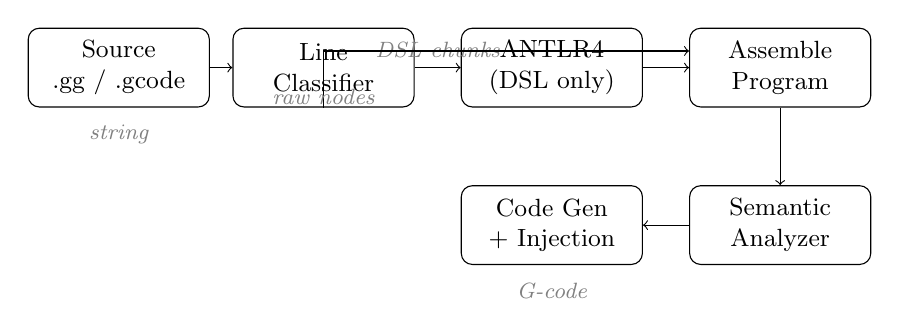
\begin{tikzpicture}[
  node distance=2.6cm,
  box/.style={draw, rounded corners, minimum width=2.3cm, minimum height=1.0cm, align=center, font=\small},
  note/.style={font=\footnotesize\itshape, text=gray}
]
\node[box] (src)  {Source\\.gg / .gcode};
\node[box] (pre)  [right of=src] {Line\\Classifier};
\node[box] (ant)  [right of=pre, node distance=2.9cm] {ANTLR4\\(DSL only)};
\node[box] (asm)  [right of=ant, node distance=2.9cm] {Assemble\\Program};
\node[box] (sem)  [below of=asm, node distance=2.0cm] {Semantic\\Analyzer};
\node[box] (gen)  [left of=sem, node distance=2.9cm] {Code Gen\\+ Injection};

\draw[->] (src) -- (pre);
\draw[->] (pre) -- node[note, above]{DSL chunks} (ant);
\draw[->] (ant) -- (asm);
\draw[->] (pre.south) |- ([yshift=6pt]asm.west) node[note, below, pos=0.25]{raw nodes};
\draw[->] (asm) -- (sem);
\draw[->] (sem) -- (gen);

\node[note] at (src.south)  [below=0.1cm] {string};
\node[note] at (gen.south)  [below=0.1cm] {G-code};
\end{tikzpicture}
\caption{Revised pipeline. Raw lines bypass ANTLR4 and are interleaved with parsed DSL statements in source order; the generator resolves anchors during code generation.}
\label{fig:m3-pipeline}
\end{figure}

% ─────────────────────────────────────────────────────────────────────────────
\section{Layer and Height Anchoring}

\subsection*{Grammar Extensions}

Three additions were made to \texttt{src/grammar/GGCode.g4}. A new keyword token \texttt{HEIGHT} was introduced, an \texttt{anchorTarget} rule expresses the two anchor flavours, and the \texttt{pauseStatement} rule was generalised. The relevant productions are:

\begin{verbatim}
pauseStatement   : PAUSE (AT anchorTarget)? ;
anchorTarget     : LAYER INTERGER   # layerAnchor
                 | HEIGHT measure   # heightAnchor ;
atBlockStatement : AT anchorTarget blockStatement ;
\end{verbatim}

The \texttt{atBlockStatement} production was wired into \texttt{compoundStatement} alongside the existing conditional, loop, and block constructs. A defensive lexer rule \verb|GCODE_COMMENT: ';' ~[\r\n]* -> skip| was also added so that any \texttt{;}-style comment surviving inside a DSL chunk is harmlessly discarded rather than causing a parse failure. The deliberate spelling \texttt{INTERGER} of the integer token, established in Chapter~2, was preserved for consistency. After editing the grammar, the parser was regenerated with the ANTLR4 tool-jar, exactly as shown in the toolchain section earlier in this chapter.

\subsection*{New AST Nodes}

The anchoring constructs are represented by two new node types and a small value object:

\begin{verbatim}
@dataclass
class Anchor:                       # value object, not a Statement
    kind: str                       # 'layer' | 'height'
    layer: Optional[int] = None
    height: Optional[float] = None  # millimetres

@dataclass
class AtBlockStatement(Statement):
    anchor: Anchor
    body: Block

@dataclass
class PauseStatement(Statement):
    anchor: Optional[Anchor] = None  # None => inline pause
\end{verbatim}

The corresponding visitor methods \texttt{visitLayerAnchor}, \texttt{visitHeightAnchor}, \texttt{visitAtBlockStatement}, and \texttt{visitPauseStatement} were added to \texttt{ASTBuilder}. Height anchors are normalised to millimetres at construction time, so \texttt{2cm} and \texttt{20mm} produce identical \texttt{Anchor} objects.

\subsection*{The \texttt{Pause} Command: A Latent-Bug Fix}

The work in this phase also corrected a defect inherited from the original implementation. The grammar contained a \texttt{pauseStatement} production, but \texttt{ASTBuilder} provided no \texttt{visitPauseStatement} override. Consequently every \texttt{Pause} statement was silently discarded by the default visitor, and no pause ever reached the generated output. Supplying the visitor, together with the generalised grammar, makes \texttt{Pause} a first-class, working command for the first time: a bare \texttt{Pause} now emits an inline \texttt{M0}, and the anchored forms are injected at the resolved position (Section~\ref{sec:m3-injection}).

\subsection*{Semantic Treatment}

The semantic analyzer was extended to recognise the new nodes. \texttt{RawGCode} is treated as opaque and passes validation unconditionally, since its content is verbatim machine code outside the language's semantic model. \texttt{AtBlockStatement} has its body analysed recursively and its anchor structurally validated (a layer index must be non-negative; a height must be strictly positive). The question of whether an anchored layer or height \emph{exists} in a given file is deliberately \emph{not} answered here: that fact is only known once the layer map has been resolved during code generation, and is reported there as a warning rather than a fatal error, in keeping with the design decision that a missing anchor must never abort a compile.

% ─────────────────────────────────────────────────────────────────────────────
\section{Two-Pass Code Generation with Injection}
\label{sec:m3-injection}

Anchored constructs introduce a non-local dependency: an \texttt{At layer 50} block written at the end of the source must emit its output near the \emph{middle} of the generated file. The code generator therefore adopts a two-pass strategy, illustrated in Figure~\ref{fig:m3-injection}.

In \textbf{Pass~A}, the generator walks the program in source order and emits the base output. As it does so it records, for each layer, the index in the output line list at which that layer begins (\texttt{layer\_anchors}), and maintains a list of $(z, \text{index})$ pairs for height resolution (\texttt{z\_anchors}). Anchors are registered both at \texttt{RawGCode} layer-marker nodes and at Z-axis moves emitted by DSL \texttt{Move} statements, so the mechanism works for fully raw files, fully authored files, and mixtures of the two. When the walk encounters an \texttt{AtBlockStatement} or an anchored \texttt{PauseStatement}, it does \emph{not} emit inline; instead it renders the construct's body into an isolated line list and appends the pair (anchor, lines) to an injection table.

In \textbf{Pass~B}, each injection's anchor is resolved to an output index --- a layer anchor maps directly through \texttt{layer\_anchors}; a height anchor maps to the first recorded $z \geq H$ --- and the rendered lines are spliced in. The splices are applied in \emph{descending} index order so that an earlier insertion does not invalidate the indices of later ones. If an anchor cannot be resolved, a message is appended to a warnings list, surfaced both on standard error and as a \verb|; WARNING:| comment near the top of the output, and the injection is skipped.

\begin{figure}[H]
\centering
\begin{tikzpicture}[
  node distance=1.0cm and 1.4cm,
  box/.style={draw, rounded corners, minimum width=3.0cm, minimum height=0.9cm, align=center, font=\small},
  small/.style={font=\footnotesize}
]
\node[box] (walk) {Pass A: walk program};
\node[box, below=of walk] (rec) {record layer / z anchors};
\node[box, right=of walk] (coll) {collect anchored\\blocks (deferred)};
\node[box, below=of rec] (res) {Pass B: resolve anchors};
\node[box, below=of res] (spl) {splice (descending index)};
\node[box, right=of spl] (warn) {unresolved $\rightarrow$ warning};

\draw[->] (walk) -- (rec);
\draw[->] (walk) -- (coll);
\draw[->] (rec) -- (res);
\draw[->] (coll) |- (res);
\draw[->] (res) -- (spl);
\draw[->] (res) -- (warn);
\end{tikzpicture}
\caption{Two-pass injection. Pass~A emits the base output and records anchors; Pass~B splices deferred blocks at their resolved positions.}
\label{fig:m3-injection}
\end{figure}

\paragraph{A note on chunk unwrapping.}
Because each DSL chunk is parsed independently, \texttt{visitProgram} wraps a chunk's statements in a single \texttt{Block}. The helper \texttt{\_parse\_dsl\_chunk} in \texttt{src/main.py} unwraps this outer block so that top-level anchored constructs sit directly in the program's statement list, where the generator's injection routing can see them. Without this step the constructs would be nested one level too deep and would be emitted inline rather than injected --- a subtlety that was diagnosed and corrected during development.

\subsection*{Worked Example}

Given the following input, in which a raw three-layer file is augmented with one anchored block and one anchored pause:

\begin{verbatim}
; layer 1, Z = 0.300
G1 X1 Y1 E0.1
; layer 2, Z = 0.500
G1 X2 Y2 E0.2
; layer 3, Z = 0.700
G1 X3 Y3 E0.3
At layer 2 { Temperature 180C }
Pause at height 0.6mm
\end{verbatim}

the compiler produces the following output. The \texttt{At layer 2} block is injected immediately after the layer-2 boundary, and the height anchor \texttt{0.6mm} resolves to layer~3 (the first layer reaching $Z \geq 0.6$):

\begin{verbatim}
; Start of GG-Code Program
; layer 1, Z = 0.300
; >> Layer 1 (Z=0.300mm)
G1 X1 Y1 E0.1
; layer 2, Z = 0.500
; >> Layer 2 (Z=0.500mm)
M104 S180 ; Set Temp
G1 X2 Y2 E0.2
; layer 3, Z = 0.700
; >> Layer 3 (Z=0.700mm)
; PAUSE at height 0.6mm
M0
G1 X3 Y3 E0.3
; End of Program
\end{verbatim}

% ─────────────────────────────────────────────────────────────────────────────
\section{Revised Module Structure}

The superset extension adds one module and revises several others. Table~\ref{tab:m3-files} lists the components touched, complementing the project structure presented in the Implementation Overview at the start of this chapter.

\begin{table}[H]
\centering
\begin{tabular}{|l|p{8.7cm}|}
\hline
\textbf{File / Directory} & \textbf{Change} \\
\hline
\texttt{src/preprocessor/line\_classifier.py} & \textbf{New.} Classifies source lines and builds the layer map; emits \texttt{RawGCode} run-nodes and DSL chunks \\
\hline
\texttt{src/grammar/GGCode.g4} & \texttt{HEIGHT} token; \texttt{anchorTarget}, \texttt{atBlockStatement}; generalised \texttt{pauseStatement}; defensive \texttt{;}-comment rule \\
\hline
\texttt{src/ast\_nodes/statements.py} & New \texttt{RawGCode}, \texttt{Anchor}, \texttt{AtBlockStatement}; redefined \texttt{PauseStatement} \\
\hline
\texttt{src/parser/antlr\_converter.py} & \texttt{visitPauseStatement}, \texttt{visitAtBlockStatement}, \texttt{visitLayerAnchor}, \texttt{visitHeightAnchor} \\
\hline
\texttt{src/main.py} & \texttt{run\_pipeline} rewired to classify-then-parse; \texttt{\_parse\_dsl\_chunk} helper \\
\hline
\texttt{src/codegen/gcode\_generator.py} & Two-pass generation with anchor recording, injection, and warnings; verbatim \texttt{RawGCode} emission \\
\hline
\texttt{src/semantic/semantic\_analyzer.py} & Validation for \texttt{RawGCode}, \texttt{AtBlockStatement}, and the new \texttt{PauseStatement} \\
\hline
\texttt{frontend/src/components/GCodeVisualizer.tsx} & Pause surfaces, layer slider, per-layer segmentation \\
\hline
\texttt{tests/test\_gcode\_superset.py} & \textbf{New.} Hypothesis-driven test suite (Section~\ref{sec:m3-validation}) \\
\hline
\end{tabular}
\caption{Modules added or revised in the superset extension}
\label{tab:m3-files}
\end{table}

% ─────────────────────────────────────────────────────────────────────────────
\section{Web IDE Enhancements}

\subsection*{Opening \texttt{.gcode} as GG-Code}

The Monaco-based editor was given a second syntax-highlighting language, \texttt{gcode}, whose tokenizer colours \texttt{G}/\texttt{M} commands, tool selects, axis and feedrate parameters, and \texttt{;} comments. When a file is uploaded, its extension is inspected: a \texttt{.gcode} file activates the \texttt{gcode} language, while a \texttt{.gg} file (or a built-in sample) uses the existing \texttt{ggcode} language. The \texttt{ggcode} tokenizer was also extended with the \texttt{HEIGHT} keyword and \texttt{mm}/\texttt{cm} measure literals introduced for anchoring. The backend required no change, as the \texttt{/upload} endpoint already returns raw file contents.

\subsection*{Visualizing Pauses}

The Three.js visualizer was extended to make pauses visible in three dimensions. The G-code parser, which previously tracked only motion, now also tracks the active layer height (from \verb|; layer| markers, the \verb|; >> Layer| annotations, and Z moves) and detects the \verb|; PAUSE| comments emitted by the generator. A checkbox toggle, ``Highlight pauses'', controls two effects: every toolpath segment on a paused layer is recoloured, and a translucent horizontal \emph{surface} is drawn across the full extent of each paused layer at its $Z$ height. The surface --- sized to the layer's own XY bounding box, with a small overhang --- communicates ``the print pauses here'' far more legibly than a point marker would.

\subsection*{The Layer Slider}

A slider ranging from $0$ to the total layer count controls how many layers, counted from the bottom upward, are rendered. This lets the user peel the model back one layer at a time to inspect interior structure and to confirm where an anchored block was injected. The paused layers are marked as ticks on the slider track at their corresponding positions, tying the temporal notion of a pause to the spatial layer-selection control.

\subsection*{A Segmentation Defect and Its Resolution}

Implementing the slider exposed a latent defect in the visualizer's path parser. The parser began a new render segment only when the G-code command \emph{type} changed between \texttt{G0} (rapid) and \texttt{G1} (linear). Real slicer output, including the reference file, frequently uses \texttt{G1} exclusively; no command change ever occurred, so the entire model collapsed into a single segment tagged with the topmost layer. The slider consequently hid the whole model except at its maximum value. The fix was to break a segment whenever the \emph{layer} changes --- on a Z move or a layer marker --- in addition to command changes. On the reference file this yields 241 segments across all 241 layers, and the slider behaves as intended.

% ─────────────────────────────────────────────────────────────────────────────
\section{Validation: A Hypothesis-Driven Evaluation}
\label{sec:m3-validation}

The superset extension was developed and assessed using an explicitly hypothesis-driven method. Five hypotheses were stated before implementation, each paired with an experiment, and the resulting test suite (\texttt{tests/test\_gcode\_superset.py}) encodes those experiments as automated checks. Table~\ref{tab:m3-hypotheses} summarises the hypotheses and outcomes.

\begin{table}[H]
\centering
\begin{tabular}{|c|p{6.0cm}|p{4.6cm}|}
\hline
\textbf{H} & \textbf{Hypothesis} & \textbf{Outcome} \\
\hline
H1 & Any raw G-code line is carried through unchanged (superset fidelity). & Confirmed: all 135{,}152 \texttt{G1} lines and every \texttt{G92}/\texttt{M}/\texttt{T} command preserved 1:1. \\
\hline
H2 & Routing only DSL through ANTLR4 keeps large files interactive. & Confirmed: 142{,}465 lines compile in $\approx 0.15$\,s. \\
\hline
H3 & \texttt{At layer/height} blocks inject at the correct position. & Confirmed by placement assertions. \\
\hline
H4 & \texttt{Pause} works end-to-end (no longer dropped). & Confirmed: regression and placement tests pass. \\
\hline
H5 & A missing anchor degrades gracefully. & Confirmed: warning emitted, compile succeeds. \\
\hline
\end{tabular}
\caption{Hypotheses and validation outcomes for the superset extension}
\label{tab:m3-hypotheses}
\end{table}

The decisive result is H2. The reference file of 142{,}465 lines compiles end-to-end in approximately $0.15$~seconds, against a target of ten seconds, while conserving the exact count of every machine command (H1). The full suite of \textbf{22} tests --- the ten pre-existing pipeline tests plus twelve new ones covering verbatim fidelity, layer-marker detection, block and inline injection placement, unit conversion (\texttt{2cm} $\rightarrow$ 20\,mm), the pause regression, mixed ordering, the missing-anchor warning, and a large-file performance check --- passes. As an end-to-end confirmation, appending \texttt{At layer 50 \{ Pause \}} to the reference file injects exactly one \texttt{M0}, positioned immediately after the \texttt{; layer 50} marker.

% ─────────────────────────────────────────────────────────────────────────────
\section{Limitations and Future Work}
\label{sec:limitations}

The GG-Code compiler is fully operational across the five pipeline stages and, with the superset extension described above, can additionally ingest, edit, and losslessly round-trip existing G-code. Programs covering temperature control, timed waits, axis movements, geometric shapes, \texttt{Repeat} loops, conditional branches, layer- and height-anchored insertion, and the \texttt{Pause} command all compile correctly and produce valid G-code. This section provides an honest assessment of the current limitations and identifies the most impactful directions for future development.

\subsection*{What Currently Works}

The following features are implemented and covered by the integration test suite in \texttt{tests/test\_pipeline.py}:

\begin{itemize}
    \item[-] All motion commands: \texttt{Move to} with axis singles, pairs, and triplets; \texttt{Home} with optional axis list.
    \item[-] Machine commands: \texttt{Temperature}, \texttt{Wait for} in seconds and minutes.
    \item[-] Geometric primitives: \texttt{Add Square}, \texttt{Add Rectangle}, \texttt{Add Circle} (segmented and exact modes), \texttt{Add Line}.
    \item[-] Control flow: \texttt{Repeat N times} (statically unrolled), \texttt{If...Then...Else} (statically evaluated).
    \item[-] Variables: \texttt{Set variable to expression} with full arithmetic expression support.
    \item[-] Named locations: \texttt{Define location as coordinates} with semantic validation.
    \item[-] Layer height tracking with automatic layer annotation comments.
    \item[-] Superset ingestion: raw \texttt{.gcode} files are opened, edited, and losslessly round-tripped.
    \item[-] Layer- and height-anchored insertion (\texttt{At layer N \{ \ldots \}}, \texttt{At height H \{ \ldots \}}) and a working \texttt{Pause} command, inline and anchored.
    \item[-] Web interface: FastAPI backend with \texttt{/compile} and \texttt{/upload} endpoints; React frontend with a dual-language Monaco editor and a Three.js 3D visualizer with pause highlighting and a layer slider.
\end{itemize}

\subsection*{Known Limitations}

\paragraph{While loops cannot be fully compiled.}
The \texttt{WhileStatement} node is handled by emitting the loop body exactly once with a warning comment, because G-code does not support runtime conditional branching. True dynamic while loops are architecturally incompatible with the compilation target. This limitation is fundamental and can only be resolved by targeting a richer output language such as Marlin's macro scripting extension.

\paragraph{Conditions are evaluated statically.}
The \texttt{IfStatement} condition is evaluated using the values stored in \texttt{self.env} at compile time. If a condition depends on a variable whose value was not set by a prior \texttt{SetStatement} (for example, it is set only inside a loop body), the variable will resolve to~0 by default, potentially emitting the wrong branch. There is no warning issued in this case.

\paragraph{No type checking in expressions.}
The expression evaluator does not distinguish between numeric and non-numeric values. Division by zero, for example, raises a Python \texttt{ZeroDivisionError} that propagates as an unhandled exception. A type-checking pass over the AST before code generation would catch these errors with proper source location information.

\paragraph{Semantic analysis collects only the first error.}
The compiler terminates at the first \texttt{SemanticError}. A batch error collection pass would allow all semantic violations to be reported together, which is significantly more useful during iterative development.

\paragraph{No feedrate on individual moves.}
The \texttt{Move to} command always emits \texttt{G1} (linear interpolation). There is currently no syntax to attach a feedrate to an individual move. The only way to set feedrate is via \texttt{Set speed to N}, which emits a standalone \texttt{G1 F\{N\}} command.

\paragraph{Height anchoring is layer-granular.}
A height anchor resolves to the first layer whose $Z$ reaches the requested value; it cannot inject \emph{within} a layer. This matches the granularity at which pauses are physically meaningful in layered manufacturing, but it means \texttt{At height 2.45mm} on a 0.2\,mm-layer print snaps to the layer boundary at $Z = 2.6$ rather than interpolating.

\paragraph{Absolute-coordinate assumption.}
Both the layer tracker and the visualizer interpret coordinates as absolute (\texttt{G90}). A file that switches to relative mode (\texttt{G91}) would mislead the layer-detection logic. Honouring the modal \texttt{G90}/\texttt{G91} state is a natural next step.

\paragraph{Arc moves are not attributed to layers.}
The visualizer tracks layers from linear (\texttt{G0}/\texttt{G1}) moves; arc commands (\texttt{G2}/\texttt{G3}) are not yet decomposed for layer attribution, so CNC programs dominated by arcs would under-report their layer structure.

\subsection*{Directions for Future Work}

\paragraph{Feedrate per move.}
Adding an optional feedrate parameter to \texttt{Move to} (e.g., \texttt{Move to X10 Y10 at 2000}) would require one new grammar rule, a field on \texttt{MoveStatement}, and a minor update to the code generator. This is a low-effort, high-impact improvement.

\paragraph{Extended machine command set.}
The current machine command set covers only temperature, wait, and tool selection. Adding fan control (\texttt{M106}/\texttt{M107}), bed temperature (\texttt{M140}/\texttt{M190}), and extruder motor control would expand the practical coverage of the language for 3D printing workflows.

\paragraph{For loop over a range.}
A \texttt{For i from 1 to N} construct would allow programs to generate indexed patterns (e.g., layers at increasing Z values) without manually unrolling. This requires additions to the grammar, a new \texttt{ForStatement} node, and a code generator pass that tracks the loop variable and emits each iteration.

\paragraph{Source-location diagnostics in the CLI.}
Both syntax errors and semantic errors carry source line and column information, but the CLI currently only prints the error message. Reporting the offending source line with a visual caret indicator (as GCC and Rust compilers do) would significantly improve the debugging experience.

\paragraph{Named toolpath procedures.}
A \texttt{Define toolpath name \{ ... \}} construct analogous to a function definition would allow the user to define reusable motion sequences and invoke them by name throughout the program. The compiler would inline the procedure body at each call site during code generation.

\paragraph{Conditional anchoring.}
A compelling extension is to allow anchored blocks to carry conditions evaluated against print metadata (for example, ``insert a purge only on layers that change tool''). This would build directly on the injection machinery introduced in this chapter, combining it with the static-evaluation model used for conditionals.
